\subsection{Database}
MySQL was selected as database service technology.

ERD schematic is presented at the figure \ref{fig:database_erd_schematic}.
\begin{figure}[h]
    \centering
    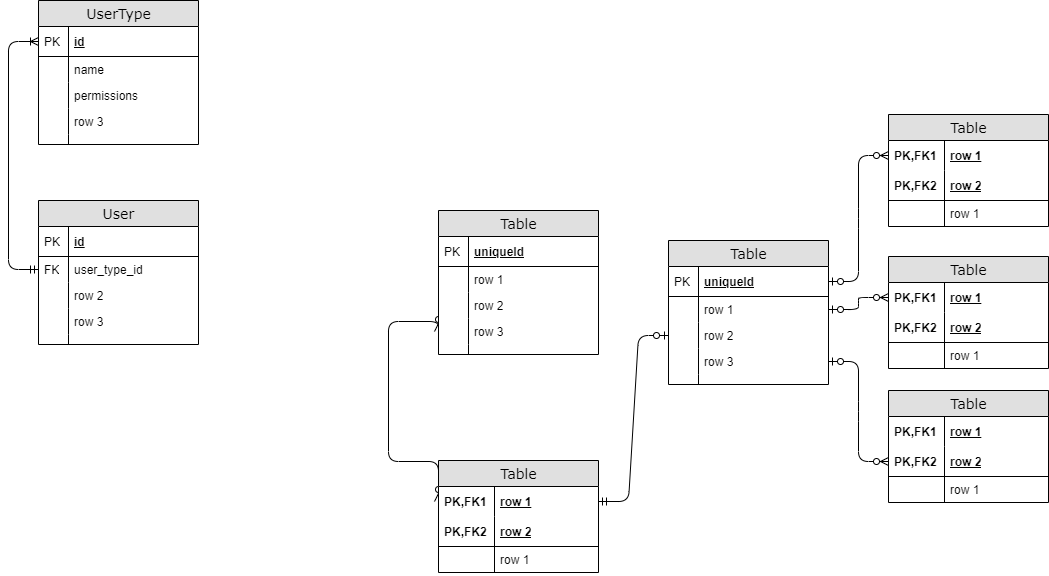
\includegraphics[width=\textwidth]{Include/Resources/Database/Project/databse_ERD_diagram.png}
    \caption{ERD schematic diagram}
    \label{fig:database_erd_schematic}
\end{figure}

Database tables:
\begin{itemize}
    \item \textit{UserType} table should be prepared before system deployment. Data from this table will be not available to change from the system.
    
    \item \textit{User} table contains user data. Each of users in the system has separated entry. User type  is defined by userTypeId that reefers to the \textit{UserType} table.
    
    \item \textit{UserToken} table contains security information about logged in users.
    
    \item \textit{BorrowedPeriod} table contains information about how long book can be borrowed by user.
    
    \item \textit{BorrowedPlace} table contains the name of place where book can be read.
    
    \item \textit{BookGenere} table contains name of the type of the book.
    
    \item \textit{CoverType} table contains all possible cover types of the books in library.
    
    \item \textit{Author} table store basic personal data of the authors of the books.
    
    \item \textit{Book} table store all books existing in library.
    
    \item \textit{Borrowed} table store all borrow orders details.
\end{itemize}
